\documentclass[10pt,twocolumn,letterpaper]{article}

\usepackage{cvpr}
\usepackage{times}
\usepackage{epsfig}
\usepackage{graphicx}
\usepackage{amsmath}
\usepackage{amssymb}

% Include other packages here, before hyperref.

% If you comment hyperref and then uncomment it, you should delete
% egpaper.aux before re-running latex.  (Or just hit 'q' on the first latex
% run, let it finish, and you should be clear).
\usepackage[breaklinks=true,bookmarks=false]{hyperref}

\cvprfinalcopy % *** Uncomment this line for the final submission

\def\cvprPaperID{****} % *** Enter the CVPR Paper ID here
\def\httilde{\mbox{\tt\raisebox{-.5ex}{\symbol{126}}}}

% Pages are numbered in submission mode, and unnumbered in camera-ready
%\ifcvprfinal\pagestyle{empty}\fi
\setcounter{page}{4321}
\begin{document}

%%%%%%%%% TITLE
\title{Anomaly detection in image data sets using deep learning}

\author{Kumar Saketh, Ali Radha\\
Department of EECS\\
University of Michigan\\
{\tt\small \{ksreddy,aliradha\}@umich.edu}
% For a paper whose authors are all at the same institution,
% omit the following lines up until the closing ``}''.
% Additional authors and addresses can be added with ``\and'',
% just like the second author.
% To save space, use either the email address or home page, not both
}

\maketitle
%\thispagestyle{empty}

%%%%%%%%% ABSTRACT
\begin{abstract}
In this project, we are interested in designing an algorithm for automatically detecting anomalies in image data sets. To get around hand-engineering features, we plan to exploit current work on deep learning to automatically extract features in an unsupervised manner. In particular, we plan to learn deep networks (in an unsupervised manner) from the unlabeled image data set of interest, and subsequently use the learned network in two different ways to detect anomalies: (i) detect anomalous images using the features learned by the network, and (ii) detect anomalous images based on the pattern generated by the active nodes  corresponding to each image.
\end{abstract}

%%%%%%%%% BODY TEXT
\section{Introduction}

Anomaly detection is the task of identifying entities in a data set which differ from the nominal majority. Anomaly detection has been studied extensively for structured multivariate data where each entity is represented by a set of $d$ features. Recently, there has been some work on solving anomaly detection for unstructured data such as time-series, network graphs and images~\cite{adsurvey} . However, most of these methods rely on extracting hand-engineered features from the unstructured data and subsequently applying anomaly detection methods for structured data.

With the advent of deep learning, feature representations can now be learned automatically from large unlabeled collections of images. It has been shown that the features inherently learned by these deep architectures have been successful in several tasks in computer vision including classification and segmentation. 

%We believe that these deep architectures can also be exploited to detect anomalous images in large image data sets. 

We are keen to build off of this work and use the features learned from deep neural networks to detect anomalous images. If we are successful, our proposed idea of using deep learning to detect anomalous images will have the advantage over traditional hand-engineering based methods in that (i) the algorithm will generalize to a wide variety of image data sets, and (ii) the performance of our algorithm, as is the case in classification tasks, could potentially be better that the performance of hand-engineered systems. For these reasons, we are excited to work on this problem.


\subsection{Current work}
There are several algorithms for detecting anomalous images using hand-engineered features~\cite{adsurvey}. Currently, the only algorithm we know of for detecting anomalies using deep networks is based on identifying images with large reconstruction errors~\cite{h2o}. The basic idea in this work is to first build an auto-encoder to learn features, and then subsequently calculate the reconstruction error for each image in the data set, and declare images with large reconstruction errors as anomalies. This method was applied to the MNIST data set in \cite{h2o} to detect 'ugly' hand-written digits.

\begin{figure*}[ht!]
\centering
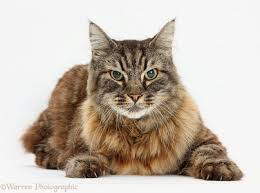
\includegraphics[width=40mm]{figs/cat1.jpeg}

\includegraphics[width=40mm]{figs/cat2.jpeg}

\includegraphics[width=40mm]{figs/cat3.jpeg}
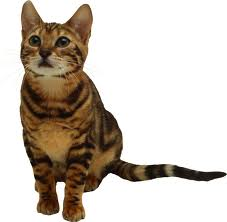
\includegraphics[width=40mm]{figs/cat4.jpeg}
\caption{Nominal cat images with no background\label{overflow}}
\end{figure*}



The method based on reconstruction errors will work well for clean image data sets such as MNIST where each image has only one object of interest (a digit in the case of MNIST), and there is no background clutter. However, for data sets where there is background noise, the reconstruction error method can fail in the following scenario - for images with nominal objects but unique background clutter, the reconstruction error can be high because of the auto-encoder model's inability to reconstruct the background. As a result, these images will be classified as anomalies. One way to view the reconstruction error based anomaly detection method is that the method is designed to detect images where any portion of the image is unique and classify them as anomalies. As a result, this method could result in a large number of false positives in data sets with varied forms of background clutter.

For instance, consider a toy data set where a majority of the images are of cats with no background, such as the ones depicted in Figure 1. Also assume that this toy data set has a few images of cats with background, like in Figure 2, and also a few images of dogs, like in Figure 3. The reconstruction based method would then classify images of dogs as anomalies as expected, but additionally, they would also classify images of cats with background as anomalies because the model will fail to reconstruct the background. Instead, we would like to design algorithms which will detect only the dog images as anomalies.

\begin{figure}[ht!]
\centering

\includegraphics[width=40mm]{figs/cat_background.jpeg}
\caption{Cat image with background\label{overflow}}
\end{figure}

\begin{figure}[ht!]
\centering
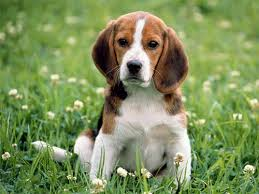
\includegraphics[width=40mm]{figs/dog.jpeg}
\caption{Dog image\label{overflow}}
\end{figure}

%-------------------------------------------------------------------------
\section{Proposed work}

To overcome the drawback of the reconstruction error based method, we propose the following. First, we make the observation that the features learned in a deep network are invariant to confounding image attributes~\cite{invariance} and therefore inherently filter out background clutter. We plan to exploit this property by detecting anomalies based on the features learned by the network as opposed to detecting anomalies based on the reconstruction error. Next, we formally describe our proposed approach.

\subsection{Framework and Approaches}
Assume a data set of unlabeled images ${\cal{I}}$ comprising of $n$ images $${\cal{I}} = \{I_1, I_2, \dots, I_n\}.$$ The goal is to detect anomalous images from this data set ${\cal{I}}$. Our proposed algorithm for detecting anomalies has the following steps:
\begin{enumerate}
\item Build a unsupervised deep network ${\cal{D}}$ to model ${\cal{I}}$. The model can either be based on auto-encoders or probabilistic networks such as deep belief networks.
\item Use the learned network to detect anomalies by adopting one of the following two alternatives:
\begin{enumerate}
\item Feed each image $I_j$ through ${\cal{D}}$, and obtain the intermediate features $F_j$ - the middle layer of auto-encoders, or the final layer of deep belief nets - with respect to ${\cal{D}}$ corresponding to $I_j$. Detect anomalies based on the features ${\cal{F}} = \{F_1, F_2, \dots\, F_n\}$ by running them through an anomaly detection algorithm for multivariate data. We plan to use the Isolation Forest algorithm~\cite{iforest}, which is currently state-of-the-art, for this purpose.
\item Feed each image $I_j$ through ${\cal{D}}$, and identify the subset of nodes $S_j$ in ${\cal{D}}$ that are activated by $I_j$. If ${\cal{D}}$ has $k$ hidden nodes,  we represent each $S_j$  as a sparse, binary k-dimensional vector with the non-zero entries in $S_j$ corresponding to the node indices of the nodes activated in ${\cal{D}}$ by $I_j$. Next, detect anomalies based on the features ${\cal{S}} = \{S_1, S_2, \dots\, S_n\}$ by running them through an anomaly detection algorithm for multivariate data.
\end{enumerate}
\end{enumerate}

In contrast with the reconstruction based method, we expect our proposed method to detect only images which are different with respect to the features learned by the deep network as anomalies. This will ensure that images with nominal objects of interest, but with unique background clutter, are not classified as anomalous. For instance, in the toy example described in Section 1, we expect our method to only detect dog images as anomalies, and recognize cat images with background as nominal.

\subsection{Software}
We are planning to use the Theano package for implementing deep networks, with Python 2.7 as the interface.


\subsection{Data sets}
We are planning to use the following two data sets:
\begin{enumerate}
\item MNIST data set~\cite{mnist}: First, we will start off by using the MNIST data set, which has images with clean black backgrounds. The goal here is to detect ugly handwritten digits. When working with MNIST, we will compare the anomalies generated by our method with the anomalies generated by the reconstruction error based method. For this data set, we expect the results generated by our method and the reconstruction error based method to be similar.
\item ImageNet data set~\cite{imagenet}: Next, we will work with the ImageNet data set. From the ImageNet data set, we will create subsets for anomaly detection task by including all images in the ImageNet data set from certain classes (for example: sky, flowers, trees), and then contaminating this data set by introducing a few images of certain other classes (for example: dogs, cats). We will not use the labels while running the algorithm, but will use the labels to evaluate the performance of our algorithm and contrast this performance with the reconstruction error based method.

% Leaving this out because 715 images might not be sufficient to train a deep network. \item Stanford Background data set~\cite{sbd}: Finally, we will work withe Stanford Background data set. This data set is unique in that all the images in the data set have labeled backgrounds in addition to labels on the foreground. Here, like in the ImageNet case, we will create subsets for anomaly detection task based on the labels of the foreground objects, and use these labels to evaluate performance. We expect our method to outperform the reconstruction error method in this case.

\end{enumerate}

\subsection{Things to learn}
In order to implement this project, we will need to learn about existing work on deep networks, and also on how to use Theano in order to implement deep networks. We will also need to learn and implement the Isolation Forest algorithm for anomaly detection.

%-------------------------------------------------------------------------
\section{Expected outcome}
If successful, we expect to have designed an automatic algorithm that is invariant to background clutter for detecting anomalies in image data sets. We will base our evaluation of whether we are successful on the MNIST data set by (i) visually eyeballing the results, and (ii) comparing our results with the existing reconstruction error based method which has been shown to be successful in identifying badly written digits. Next, we will base our evaluation of success on the ImageNet data set by utilizing the labels available in the data set, specifically in the form of ROC's~\cite{roc}. We would consider our proposed method to be a success if we obtain a high value for the area under the ROC curve (AUC), and if we outperform the reconstruction error based method with respect to the AUC.

The components that we think are risky are the following:
\vspace{-0.1in}
\begin{enumerate}
\item Inability to successfully train a deep network: Training deep networks is tricky~\cite{tricky}. Furthermore, we will need significant computing resources to train large networks, which might be hard to obtain from the university.
\item Anomaly detection on high-dimensional data: The features learned from the deep networks, or the node activation patterns, could be fairly high-dimensional. Detecting anomalies in high dimensional data accurately could be hard because of the curse of dimensionality. 
\item Potentially incorrect hypothesis: Our hypothesis that our method will work better than the reconstruction error based method could potentially fail to hold in practice, in which case we might not get a significant improvement over the reconstruction error based method.
\end{enumerate}

We are confident that we will be able to build auto-encoders by following the tutorial by Andrew Ng~\cite{ufldl}. Therefore, the least we expect to deliver, subject to the risky items failing, is reproducing the reconstruction error based method~\cite{h2o} and its results on the MNIST data set. If we are successful in training DBN's, we will then have an alternative deep network structure to the auto-encoders off which we can detect anomalies by comparing the likelihood instead of comparing the reconstruction error as is the case with auto-encoders. If we are successful in getting the anomaly detection method to work, either by limiting the dimension of the feature space ${\cal{F}}$ or by exploiting the sparse nature of ${\cal{S}}$, we should have a working algorithm that should at the very least work as well as the reconstruction error based method, if not better.

%-------------------------------------------------------------------------

\small{
\begin{thebibliography}{1}

\bibitem{adsurvey}
Chandola, Varun, Arindam Banerjee, and Vipin Kumar. "Anomaly detection: A survey." ACM Computing Surveys (CSUR) 41.3 (2009): 15.
\bibitem{h2o}
\url{http://learn.h2o.ai/content/hands-on_training/anomaly_detection.html}

\bibitem{invariance}
Goodfellow, Ian, et al. "Measuring invariances in deep networks." Advances in neural information processing systems. 2009.

\bibitem{iforest}
Liu, Fei Tony, Kai Ming Ting, and Zhi-Hua Zhou. "Isolation forest." Data Mining, 2008. ICDM'08. Eighth IEEE International Conference on. IEEE, 2008.

\bibitem{mnist}
LeCun, Yann, and Corinna Cortes. "The MNIST database of handwritten digits." (1998).

\bibitem{imagenet}
Deng, Jia, et al. "Imagenet: A large-scale hierarchical image database." Computer Vision and Pattern Recognition, 2009. CVPR 2009. IEEE Conference on. IEEE, 2009.

%\bibitem{sbd}
%Ren, Xiaofeng, Liefeng Bo, and Dieter Fox. "Rgb-(d) scene labeling: Features and algorithms." Computer Vision and Pattern %Recognition (CVPR), 2012 IEEE Conference on. IEEE, 2012.

\bibitem{roc}
Hanley, James A., and Barbara J. McNeil. "The meaning and use of the area under a receiver operating characteristic (ROC) curve." Radiology 143.1 (1982): 29-36.

\bibitem{tricky}
Hinton, Geoffrey. "A practical guide to training restricted Boltzmann machines." Momentum 9.1 (2010): 926.

\bibitem{ufldl}
Ng, Andrew, et al. "UFLDL tutorial." (2012).
\end{thebibliography}
}

\end{document}
